\documentclass[12pt]{article}
\usepackage{amsmath}
\usepackage{mathtools}
\usepackage{graphics,epsfig}
\usepackage{xspace}
\usepackage{color}
\usepackage{amssymb}
\usepackage{subfigure}
\usepackage{multirow}
\usepackage{listings}
\usepackage{url}

\usepackage[noend]{algpseudocode}
\usepackage{algorithmicx,algorithm}

%%uncomment following line if you are going to use ``Chinese''
% \usepackage{ctex} 

\definecolor{ballblue}{rgb}{0.13, 0.67, 0.8}
\definecolor{cornflowerblue}{rgb}{0.39,0.58,0.93}
\definecolor{babyblueeyes}{rgb}{0.63, 0.79, 0.95}

% preset-listing options
% preset-listing options
\lstset{
	backgroundcolor=\color{white},   
	basicstyle=\footnotesize,    
	language=matlab,
	breakatwhitespace=false,         
	breaklines=true,                 % sets automatic line breaking
	captionpos=b,                    % sets the caption-position to bottom
	commentstyle=\color{ballblue},    % comment style
	extendedchars=true,              
	frame=single,                    % adds a frame around the code
	keepspaces=true,                 
	keywordstyle=\color{blue},       % keyword style
	numbers=left,                    
	numbersep=5pt,                   
	rulecolor=\color{babyblueeyes},
	stepnumber=1,              
	stringstyle=\color{black},     % string literal style
	tabsize=4,                       % sets default tabsize to 4 spaces
	title=\lstname                   
}

\lstdefinestyle{MatlabStyle}{
	language        =   Matlab, 
	keywordstyle    =   \color{blue},
	keywordstyle    =   [2] \color{teal},
	stringstyle     =   \color{magenta},
	commentstyle    =   \color{red}\ttfamily,
	breaklines      =   true,
	columns         =   fixed,
	basewidth       =   0.5em,
}


\usepackage{geometry}
\geometry{
 a4paper,
 total={210mm,297mm},
 left=20mm,
 right=20mm,
 top=20mm,
 bottom=20mm,
 }

\marginparwidth = 10pt

\graphicspath{ {images/} }

\begin{document}
\title{Course Project Report: Advanced Math Analysis with Matlab}
\author{KeZheng Xiong \\ 22920202204622}

\maketitle

\abstract{The report for the end-of-term project of Advanced Math Analysis with MATLAB fall 2021 course. All the source code is open-sourced on the Github repository \url{https://github.com/SmartPolarBear/matlab-math-analysis-csxmu-2021} under \textbf{GPLv3} license}

\tableofcontents

\pagebreak

\section{Problem 1}

\subsection{Problem Description}
Given function $F(x, y) = 0.2x^2 + 0.1y^2 + sin(x + y)$, please work out its
gradient. Based on the gradient, please find out the local extreme of function F(x,y)
when both x and y are in the range of $[-2*\pi, 2*\pi]$. The 2D and 3D views of the function
is given in Fig. 1. 

\subsection{Solution}

\subsubsection{The gradient of the function}

I get the gradient of the function using the following code

\begin{lstlisting}[style=MatlabStyle,caption=Gradient Calculation]
	syms x y;
	f=0.2*x^2+0.1*y^2+sin(x+y);
	diff(f,x)
	diff(f,y)
\end{lstlisting}

Based on the result, the gradient is

\begin{equation}
	\nabla \cdot f(x,y)=( \frac{2*x}{5} + cos(x + y), \frac{y}{5} + cos(x + y))
\end{equation}

\subsubsection{Find the extreme values}
To find the extreme values of $F(x,y)$ with gradient decent method, we walk little steps towards the direction of the gradient. To formalize this idea, the algorithm is shown as follows.

\begin{algorithm}
	\caption{Gradient Descent}
	\hspace*{0.02in} {\bf Input:}
	Initial point $x_0$, a constant $\alpha$, $k=0$
	\begin{algorithmic}
	\While{termiation condition does not hold}
	\State $k=k+1$
	\State $x_{k+1}=x_k-\alpha \nabla \cdot f(x_k)$
	
	\EndWhile
	\end{algorithmic}
\end{algorithm}

Various problems occurs if this brute-force algorithm is implemented directly. The speed of convergence is annoyingly slow if parameters are not chosen right. In fact, I never succeeded finding a set of parameters that works. A well-known optimization  called Stochastic gradient descent, or SGD, improves the performance significantly.

In the brute-force algorithm, The given parameter $\alpha$ controls how long a step is from the point $\mathbf{x_0}$ towards the direction of the gradient. It is a fixed value. On the contrary, in SGD gradient descent algorithm, the length of a step , $m$ , which is also referred to as "learning rate", will be changed each round according to the current position. To be more exact, SGD algorithm tries to find a learning rate $m$, so that it can minimize the function

\begin{equation}
	h(x,y,m) = \mathbf{x_0} + \nabla \cdot f(x,y)
\end{equation}

So, in the implementation of the algorithm, the following equation is solved each round in the while-loop to get the expected $m$ value

\begin{equation}
	\frac{\partial h}{\partial m} = 0
\end{equation}

The implementation is shown in Code \ref{code:sgd}. There are four results of the function. $endp$ is the final point, or the result of gradient descent algorithm. $num$ is the number of steps taken. $hist$ is a vector which records all the coordinates of each step, and $list$ contains the corresponding function values. The three parameters are the function, the initial point and the precision, respectively.

\begin{lstlisting}[style=MatlabStyle,caption=SGD Gradient Descent,label=code:sgd]

	function [endp,num,hist,list]=gradient_descent(f,x0,eps)
		syms x y m;
		d=-[diff(f,x);diff(f,y)];
		
		nd=subs(d,x,x0(1));
		nd=subs(nd,y,x0(2));
		nrm=double(norm(nd));
		
		list=[];
		
		k=0;
		while(nrm>=eps)
		nx0=x0+m*nd;
		nf=subs(f,x,nx0(1));
		nf=subs(nf,y,nx0(2));
		h=diff(nf,m);
		nm=solve(h);
		
		x0=x0+nm*nd;
		k=k+1;
		
		hist(k,:)=[double(x0(1));double(x0(2))];
		vf=subs(f,x,x0(1));
		vf=subs(vf,y,x0(2));
		list = [list double(eval(vf))];
		
		nd=subs(d,x,x0(1));
		nd=subs(nd,y,x0(2)); 
		nrm=double(norm(nd));
		end
		
		num=k;
		endp=x0;
	end
\end{lstlisting}

To test the implementation, Each point of the steps taken in the procedure of gradient descent algorithm is plotted on Figure \ref{fig:p1_visualize_in_contour}, in red scattered lines, and the result is in Table \ref{table:p1result}. In Table \ref{table:p1result}, the 4th column shows the value from the builtin $fminsearch$ function, which reveals that the implementation of SGD gradient descent algorithm gives the right answers.

\begin{figure}[h]
	\caption{The visualization of the steps of the SGD gradient descent algorithm}
	\centering
	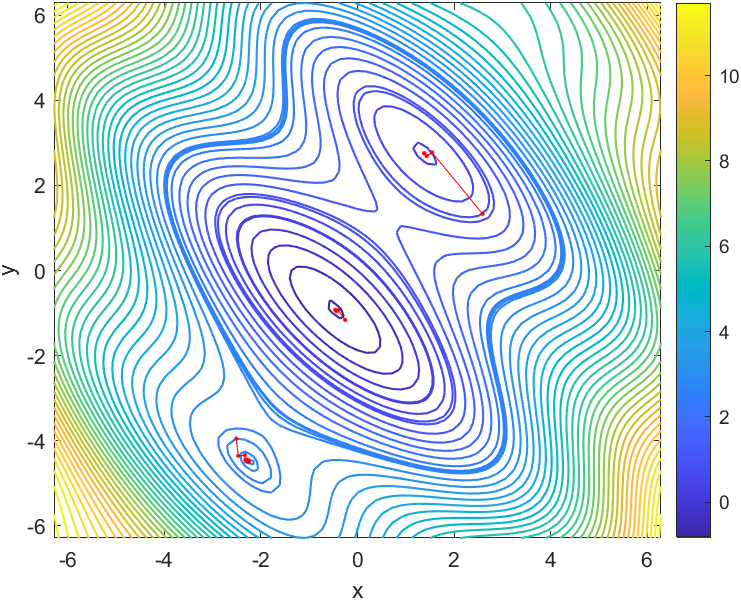
\includegraphics{p1_visualize_in_contour.png}
	
	\label{fig:p1_visualize_in_contour}
\end{figure}

The initial points for gradient descent chosen are $(-3,-4)$, $(0,-1)$, and $(-2,-2)$. The choice of initial points are significant. It can \textbf{influence the speed of convergence dramatically}. Given a bad initial point, the algorithm may not reach the point of convergence at all, or take a unbearable long time to reach there. It worth mentioning that the second choice of $(0,-1)$ is especially difficult. It takes a great many attempts to find this point which contributes to a high speed of convergence.


\begin{table}[h]
	\caption{The Extreme Values of $F(x,y)$}
	\begin{center}
		\begin{tabular}{|c|c|c|c|}
			\hline
			No. & X-Y Coordinates & $F(x,y)$ & Result of $fminsearch()$ \\ \hline
			0 & $(-2.2469,-4.4902)$ & 2.5874 &  2.5874 \\ \hline
			1 & $(-0.4611,-0.9241)$ & -0.8549 & -0.8549 \\ \hline
			2 & $(1.3768,2.7529)$ & 0.3020 & 0.3020 \\ \hline
		\end{tabular}
	\end{center}
	\label{table:p1result}
\end{table}

\subsection{Analysis and Conclusion}   
  

Gradient descent is a widely-used way of finding the extreme values of any function. There are many optimizations for this method, which will improve the speed of convergence. SGD is taken in this project, which yields satisfying results.

SGD gradient descent has a major flaw that it is known for "easy to be trapped in a local minimum", which may account for the difficulties in finding a good initial point for the second extreme value. More sophisticated optimization such as Momentum gradient descent and AdaGrad gradient descent can be applied if the speed of convergence is too slow.


\section{Problem 2}

\subsection{Problem Description}

A factory supplies engine for its customer. According to the contract, the
factory should deliver its product to the customer in the end of the 1st season: 40 engines;
in the end of the 2nd season: 60 engines; in the end of the 3rd season: 80 engines. Due
to limited productivity, to its most, the factory is only able to produce 100 machines
in a single season. The production cost is given as $f(x) = 50x + 0.2x^2$
, where $x$ is the
number of machines produced in one season. It is possible to produce machines more
than the required quota in each season. In this case, the storage cost is 4 dollars for one
machine/season. Assuming there is no reservations at the beginning for the first season,
please work out a production plan that minimizes the production cost

\subsection{Solution}

\subsubsection{The Cost Function}

Let $x_1$, $x_2$ and $x_3$ be the number of machines produced in season 1, 2 and 3, respectively.

Firstly, the production cost $P(\mathbf{x})$ is the sum of each season's production cost.

\begin{equation}
	P(\mathbf{x})=0.2(x_1^2+x_2^2+x_3^2)+50(x_1+x_2+x_3)
\end{equation}

Secondly, there are costs for storage if more machines than the need is produced each season, so the storage cost  $S(\mathbf{x})$ is the sum of each season's storage cost.

\begin{equation}
	\begin{aligned}
		S(\mathbf{x})=4*(x_1+(x_1+x_2-40)+(x_1+x_2+x_3-(40+60))) \\
		=12x_1+8x_2+4x_3-560
	\end{aligned}
\end{equation}

The total cost, say $F(\mathbf{x})$ is the sum of $P(\mathbf{x})$ and $S(\mathbf{x})$ 

\begin{equation}
	F(\mathbf{x})=0.2(x_1^2+x_2^2+x_3^2)+62x_1+58x_2+54x_3-560
\end{equation}

According to the requirements for MATLAB to solve a quadratic programming problem, function $G(x)$ is defined as follows:

\begin{equation}
\begin{aligned}
	F(\mathbf{x})=G(\mathbf{x})-560  \\
\end{aligned}
\end{equation}

And it can be standardize:

\begin{equation}
\begin{aligned}
		G(\mathbf{x})=\frac{1}{2}\mathbf{x}\mathbf{H}\mathbf{x^T}+ \mathbf{f^T}\mathbf{x} \\
	H=\left(   
	\begin{array}{ccc} 
		0.4 & 0 & 0\\
		0 & 0.4 & 0\\ 
		0 & 0 & 0.4\\ 
	\end{array}
	\right) \\
	f^T=\left(   
	\begin{array}{ccc} 
		62 & 58 & 54\\
	\end{array}
	\right) \\
\end{aligned}
\end{equation}

\subsubsection{The Constraints}

The most obvious constraints come from the max production limit.

\begin{equation}
	\begin{aligned}
	0 \le x_1 \le 100 \\
	0 \le x_2 \le 100 \\
	0 \le x_3 \le 100 \\
	\end{aligned}
\end{equation}

Write it in the form for MATLAB to solve

\begin{equation}
\begin{aligned}
	\mathbf{lb} \le \mathbf{x} \le \mathbf{ub} \\
	lb^T=\left(   
	\begin{array}{ccc} 
		0 & 0 & 0\\
	\end{array}
	\right) \\
	ub^T=\left(   
	\begin{array}{ccc} 
		100 & 100 & 100\\
	\end{array}
	\right) \\
\end{aligned}
\end{equation}

To meet the requirements of the contract, $x_1$ and $x_2$ should be enough to be delivered, and the total production $x_1+x_2+x_3$ should be just right for the total demand $40+80+100$

So we have

\begin{equation}
	\begin{aligned}
	\mathbf{A} \mathbf{x} \ge \mathbf{b}\\
	\mathbf{A_{eq}} \mathbf{x} = \mathbf{b_{eq}}
	\end{aligned}
\end{equation}

Where

\begin{equation}
\begin{aligned}
	A=\left(   
	\begin{array}{ccc} 
		1 & 0 & 0\\
		1 & 1 & 0\\ 
	\end{array}
	\right) \\
	b=\left(   
	\begin{array}{c} 
		60\\
		100
	\end{array}
	\right) \\
\end{aligned}
\end{equation}

And

\begin{equation}
	\begin{aligned}
		A=\left(   
		\begin{array}{ccc} 
			1 & 1 & 1\\ 
		\end{array}
		\right) \\
		b=\left(   
		\begin{array}{c} 
			180\\
		\end{array}
		\right) \\
	\end{aligned}
\end{equation}

\subsubsection{Code}

Now that we have translated the problem into equations and inequalities and have written them in the standard form for $quadprog()$ in MATLAB to solve, the solution can be easily implemented in Code \ref{code:p2}.

\begin{lstlisting}[style=MatlabStyle,caption=SGD Gradient Descent,label=code:p2]
\end{lstlisting}

\section{Problem 3}

\subsection{Problem Description}
\textbf{Prove:} Among the top 32 World Cup finals, the information entropy of the event that a team winning is 5.

\subsection{Proof}

The definition of information entropy by Shannon is

\begin{equation}
	H(X)=-\sum_{i}P(x_i)log_2(P(x_i))
\end{equation}

Let $p_i$ be the possibility for team $i$ to win, the Shannon entropy $H$ is

\begin{equation}
	H(X)=-\sum_{i=1}^{32}P(x_i)log_2(P(x_i))
\end{equation}

Subject to the nature of possibility, the following constraints should be satisfied.

\begin{equation}
	P(x_i) \ge 0
\end{equation}

And

\begin{equation}
	\sum_{i=0}^{32}P(x_i) = 1
\end{equation}

$H(X)$ is a multivariate function. Though it has too many variables to be plotted, it is possible to see how it scales by acquiring its maximums and minimums. To achieve this, Lagrangian multiplier method is used to implement Code \ref{code:p3}.

\begin{lstlisting}[style=MatlabStyle,caption=Get the maximum for $H(x)$,label=code:p3]
clear;
% define 32 symbols
p=sym('p',[1,32]);

% construct f, the Shannon entropy. and sum, the sum of all posibilities, which should be 1, as a constraint
f=p(1)*log2(p(1));
sum=p(1);

for i=p(2:32)
f=f+i*log2(i);
sum=sum+i;
end

f=-f;

syms r

l=f+r*(sum-1);

% get the partial derivative for each symbol
eqns=[];
for i=p
eqns=[eqns diff(l,i)];
end

eqns=[eqns diff(l,r)];
vars=[p r];

solution=solve(eqns,vars);

ps=subs(p,solution);
fs=subs(f,solution);

% output the result
format rat;
ps
eval(fs)
\end{lstlisting}

The result of Code \ref{code:p3} is that

\begin{equation}
	H(x)=5  \iff  p_i=0.03125, i=1,2,3,...,32
\end{equation}

Therefore, the proposition is proved. Among the top 32 World Cup finals, the information entropy of the event that a team winning is 5 when the possibility for each team to win is equal. The entropy will be less than 5 otherwise.
\section{Acknowledgment}

Thanks to (TODO)


\end{document}
